\chapter{Fundamentação Teórica}
\label{cap:fund}

%% - - - - - - - - - - - - - - - - - - - - - - - - - - - - - - - - - - -
\section{Aprendizado por Reforço}
\label{sec:rl}

O Aprendizado por Reforço (Reinforcement Learning - RL) é uma área do aprendizado de máquina que se concentra em agentes que aprendem a tomar decisões através da interação com um ambiente. Diferente do Aprendizado Supervisionado e do Aprendizado Não Supervisionado, o RL depende principalmente de feedback em forma de recompensas obtidas através das interações que o agente realiza no ambiente.

\subsection{Fundamentos e conceitos básicos de Aprendizado por Reforço}
\label{subsec:rl_fund}

O Aprendizado por Reforço é estruturado em torno de conceitos fundamentais que estabelecem como agentes podem aprender através da interação com o ambiente. Esta área combina elementos de programação dinâmica, teoria de controle e aprendizado estatístico para desenvolver algoritmos que permitem que agentes aprendam comportamentos ótimos através de tentativa e erro.

Os principais componentes do Aprendizado por Reforço são:

\begin{itemize}
\item \textbf{Agente}: A entidade que aprende e toma decisões. Ele observa o estado atual do ambiente, escolhe ações para executar e recebe feedback na forma de recompensas.

\item \textbf{Ambiente}: O mundo com o qual o agente interage. Ele fornece observações ao agente e responde às suas ações, gerando novos estados e recompensas.

\item \textbf{Estado}: A representação da situação atual do ambiente. O estado pode ser completamente ou parcialmente observável pelo agente.

\item \textbf{Ação}: As possíveis decisões que o agente pode tomar em cada estado. O conjunto de ações pode ser discreto ou contínuo.

\item \textbf{Recompensa}: O feedback numérico que o agente recebe após cada ação. É um sinal escalar que indica o quão boa foi uma ação tomada em um determinado estado. O objetivo do agente é maximizar a soma das recompensas ao longo do tempo.

\item \textbf{Política}: A estratégia que o agente usa para escolher ações com base no estado atual. Pode ser determinística ou estocástica.
\end{itemize}

O processo de aprendizagem no RL pode ser descrito pela seguinte sequência:

\begin{enumerate}
\item O agente observa o estado atual do ambiente.
\item Com base nesse estado, o agente escolhe uma ação.
\item O ambiente transita para um novo estado como resultado da ação.
\item O agente recebe uma recompensa associada à transição.
\item O agente atualiza sua política de decisão com base na experiência adquirida.
\end{enumerate}

Este processo é frequentemente modelado como um Processo de Decisão de Markov (MDP).

Existem alguns principais abordagens para o RL, incluindo:

\begin{itemize}
\item \textbf{Métodos baseados em valor}: Aprendem a função valor-ação \textbf{Q(s,a)}.
\item \textbf{Métodos baseados em política}: Otimizam diretamente a política \textbf{$\pi$}.
\item \textbf{Métodos ator-crítico}: Combinam estimativas de valor e otimização de política.
\end{itemize}

\subsubsection{Processo de Decisão de Markov (MDP)}
\label{subsubsec:mdp}

Os Processos de Decisão de Markov (MDPs) são um modelo matemático fundamental no aprendizado por reforço, utilizado para modelar situações onde é necessário tomar decisões sequenciais em ambientes com incerteza \cite{introducao_modelos_probabilisticos}. A Figura \ref{fig:mdp_ilustracao} ilustra um exemplo de MDP. Os MDPs possuem as seguintes características principais:

\begin{itemize}
\item \textbf{Estados (S)}: Representam as possíveis situações do ambiente.
\item \textbf{Ações (A)}: Conjunto de decisões que o agente pode tomar em cada estado.
\item \textbf{Função de transição P(s'|s,a)}: Probabilidade de transição para o estado s' dado que a ação a foi tomada no estado s.
\item \textbf{Função de recompensa R(s,a,s')}: Retorno numérico recebido ao realizar a transição de s para s' tomando a ação a.
\item \textbf{Fator de desconto γ}: Valor entre 0 e 1 que representa a importância de recompensas futuras.
\end{itemize}

Um MDP é formalmente definido como uma tupla (S, A, P, R, γ), onde:

\begin{itemize}
\item S é o conjunto de estados
\item A é o conjunto de ações
\item P : S × A × S → [0, 1] é a função de transição
\item R : S × A × S → ℝ é a função de recompensa
\item γ ∈ [0, 1] é o fator de desconto
\end{itemize}

O objetivo em um MDP é encontrar uma política ótima π* que maximize o retorno esperado:

$$ π* = \arg\max_π \mathbb{E}\left[\sum_{t=0}^{\infty} γ^t R(s_t, a_t, s_{t+1}) | π\right] $$

onde π : S → A é uma política que mapeia estados para ações.

\begin{figure}[H]
 \centering
 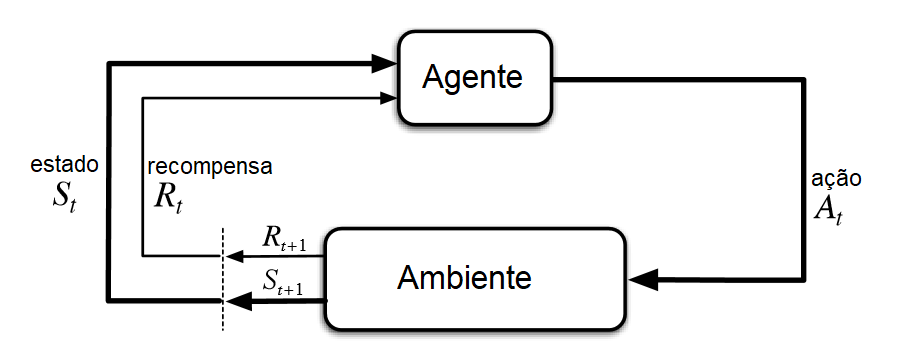
\includegraphics[width=0.60\textwidth]{fig/MDP.png}
 \caption{Exemplo de um Processo de Decisão de Markov (MDP).}
 \label{fig:mdp_ilustracao}
\end{figure}

Uma característica fundamental dos MDPs é a propriedade de Markov, que estabelece que a probabilidade de transição para um novo estado depende apenas do estado atual e da ação tomada, não dependendo de estados ou ações anteriores \cite{sutton}.

Os MDPs são amplamente utilizados em diversas áreas, incluindo:

\begin{itemize}
\item Robótica e controle automático
\item Planejamento de trajetórias
\item Gestão de recursos
\item Sistemas de recomendação
\item Jogos e simulações
\end{itemize}

Existem várias extensões dos MDPs para lidar com diferentes cenários:

\begin{itemize}
\item \textbf{POMDPs (Partially Observable MDPs)}: Lidam com situações onde o estado não é completamente observável.
\item \textbf{LLMDPs (Language-Limited MDPs)}: Incorporam restrições de linguagem nas ações e observações consideradas \cite{introducao_modelos_probabilisticos}.
\end{itemize}

Os MDPs fornecem uma base teórica sólida para o desenvolvimento de algoritmos de aprendizado por reforço, permitindo a modelagem e solução de problemas complexos de tomada de decisão sequencial sob incerteza.

\subsubsection{Funções de valor e política}
\label{subsubsec:valor_politica}

As funções de valor e política são conceitos fundamentais no aprendizado por reforço (RL), desempenhando papéis cruciais na tomada de decisões e na avaliação de estratégias. As funções de valor estimam o quão vantajoso é para um agente estar em um determinado estado ou executar uma ação específica em um estado. Existem dois tipos principais de funções de valor: a Função de Valor de Estado (V-function) e a Função de Valor de Ação (Q-function).

A Função de Valor de Estado, representada como \( V^\pi(s) \), indica o valor esperado de estar em um estado específico seguindo uma política \(\pi\). Matematicamente, é definida como \( V^\pi(s) = \mathbb{E}_\pi[G_t | S_t = s] \), onde \( G_t \) é o retorno acumulado a partir do tempo \( t \). Por outro lado, a Função de Valor de Ação, representada como \( Q^\pi(s,a) \), indica o valor esperado de tomar uma ação específica em um estado específico e depois seguir uma política \(\pi\). Sua definição matemática é \( Q^\pi(s,a) = \mathbb{E}_\pi[G_t | S_t = s, A_t = a] \).

Essas funções de valor são essenciais para métodos baseados em valor, como Q-learning e DQN (Deep Q-Network) \cite{0fe19b1631b60807bffb7757865b184d797c3016}. Elas permitem que o agente avalie a qualidade das ações em diferentes estados, facilitando a tomada de decisões ótimas.

As funções de política, por sua vez, definem o comportamento do agente, mapeando estados para ações. Existem dois tipos principais de políticas: a Política Determinística e a Política Estocástica. A Política Determinística mapeia cada estado para uma única ação, representada como \(\pi(s) = a\). Já a Política Estocástica mapeia cada estado para uma distribuição de probabilidade sobre as ações, representada como \(\pi(a|s) = P(A_t = a | S_t = s)\).

As funções de política são centrais para métodos baseados em política, como Policy Gradient e PPO (Proximal Policy Optimization) \cite{0fe19b1631b60807bffb7757865b184d797c3016}. Elas permitem que o agente aprenda diretamente qual ação tomar em cada estado, sem necessariamente estimar valores de estado ou ação.

A relação entre funções de valor e política é estreita. A função de valor avalia a qualidade de uma política, enquanto a política pode ser derivada da função de valor, por exemplo, escolhendo a ação com o maior valor \( Q \) em cada estado. Alguns métodos, como os algoritmos ator-crítico, combinam ambos os conceitos: o "ator" (política) decide quais ações tomar, e o "crítico" (função de valor) avalia essas ações e fornece feedback para melhorar a política \cite{0fe19b1631b60807bffb7757865b184d797c3016}.

O objetivo do RL é encontrar a política ótima \(\pi^*\) que maximize o retorno esperado. Isso pode ser alcançado de várias maneiras: métodos baseados em valor aprendem a função de valor ótima e derivam a política ótima a partir dela \cite{54807143779fa04466a0b0d01f4d1ecc94eb39ae}; métodos baseados em política otimizam diretamente a política, muitas vezes usando gradientes de política \cite{0fe19b1631b60807bffb7757865b184d797c3016}; e métodos híbridos combinam aprendizado de valor e otimização de política, como em algoritmos ator-crítico \cite{1911.04094}.

Recentes avanços incluem o uso de redes neurais profundas para aproximar funções de valor e política em ambientes complexos, como demonstrado no jogo de Hex \cite{54807143779fa04466a0b0d01f4d1ecc94eb39ae}, e o desenvolvimento de métodos robustos para lidar com incertezas e riscos em ambientes desafiadores \cite{2312.00342}.

As funções de valor e política são elementos cruciais no aprendizado por reforço (RL), especialmente em algoritmos avançados como o Proximal Policy Optimization (PPO). No PPO, as funções de valor são utilizadas para estimar a vantagem, que é essencial para o processo de otimização da política. A política, por sua vez, é ajustada para maximizar uma função objetivo surrogate, garantindo que as atualizações sejam estáveis e eficientes. Essa interação entre funções de valor e política permite que o PPO aprenda de forma eficaz em ambientes complexos, equilibrando desempenho e estabilidade. Vamos explorar esses conceitos e sua relação com o PPO.


\subsection{Aprendizado por Reforço Profundo}
\label{subsec:deep_rl}

O Aprendizado por Reforço Profundo (Deep Reinforcement Learning - DRL) é uma abordagem avançada de aprendizado de máquina que combina os princípios do aprendizado por reforço tradicional com as capacidades das redes neurais profundas. Esta técnica tem ganhado destaque significativo nos últimos anos devido à sua eficácia em resolver problemas complexos de tomada de decisão sequencial.

O Aprendizado por Reforço Profundo é um paradigma de aprendizado de máquina no qual um agente aprende a tomar decisões ótimas através da interação com um ambiente, utilizando redes neurais profundas para representar e processar informações complexas \cite{https://www.semanticscholar.org/paper/3879ab51e5eea7ce06dc31edbb169afb76e0bd71,https://www.semanticscholar.org/paper/45ae19e1e9037e10e90423b536eb183dcd99bd2e}. O objetivo principal é maximizar uma recompensa cumulativa ao longo do tempo, permitindo que o agente aprenda políticas de ação eficazes em ambientes dinâmicos e de alta dimensionalidade.

Uma característica fundamental do DRL é o aprendizado baseado em experiência. O agente aprende através da interação direta com o ambiente, acumulando experiência ao longo do tempo \cite{https://www.semanticscholar.org/paper/8efe27f4a31ebb72e9b3047107a4fe940259aad9}. As decisões são tomadas com base em um processo de tentativa e erro, onde o agente explora diferentes ações e aprende com os resultados obtidos.

Além disso, o DRL utiliza redes neurais profundas para processar e representar informações de alta dimensionalidade, como imagens ou dados sensoriais complexos \cite{https://www.semanticscholar.org/paper/8efe27f4a31ebb72e9b3047107a4fe940259aad9,https://www.semanticscholar.org/paper/3340124e85d6e5fbc08db49ad3e6a8d9ffa04222}. Isso permite a extração automática de características relevantes do ambiente, eliminando a necessidade de engenharia manual de recursos.

Outra característica importante é a adaptabilidade. O agente pode se adaptar a mudanças no ambiente e generalizar seu aprendizado para situações não vistas anteriormente \cite{https://www.semanticscholar.org/paper/27c834620d2c6adb51dffc4be9907e185907ce12}. O DRL é capaz de lidar com problemas parcialmente observáveis, onde nem toda a informação sobre o estado do ambiente está disponível.

O DRL também foca na otimização de longo prazo, buscando maximizar a recompensa cumulativa ao longo do tempo, em vez de apenas recompensas imediatas \cite{https://www.semanticscholar.org/paper/45ae19e1e9037e10e90423b536eb183dcd99bd2e}. Isso permite o aprendizado de estratégias complexas que envolvem planejamento e tomada de decisão em múltiplos passos.

Um dos desafios do DRL é balancear a necessidade de explorar novas ações para descobrir melhores estratégias com a exploração de ações conhecidas que já produzem bons resultados \cite{https://www.semanticscholar.org/paper/fef82649815694167ef56929648a51f2eb0849e9}. Técnicas como ε-greedy ou amostragem de Thompson são utilizadas para gerenciar este trade-off.

O Aprendizado por Reforço Profundo tem sido aplicado com sucesso em diversas áreas, incluindo navegação autônoma de robôs e veículos \cite{https://www.semanticscholar.org/paper/3340124e85d6e5fbc08db49ad3e6a8d9ffa04222,https://www.semanticscholar.org/paper/fef82649815694167ef56929648a51f2eb0849e9}, jogos eletrônicos e simulações complexas \cite{https://www.semanticscholar.org/paper/3879ab51e5eea7ce06dc31edbb169afb76e0bd71}, otimização de sistemas de controle industrial \cite{https://www.semanticscholar.org/paper/27c834620d2c6adb51dffc4be9907e185907ce12}, negociação automatizada em mercados financeiros \cite{https://www.semanticscholar.org/paper/45ae19e1e9037e10e90423b536eb183dcd99bd2e}, e gerenciamento de redes de comunicação e IoT \cite{https://www.semanticscholar.org/paper/3879ab51e5eea7ce06dc31edbb169afb76e0bd71,https://www.semanticscholar.org/paper/668a75bdb9c3f6d088f7da2b4b76ec1e66c484b8}.

Apesar de seu potencial, o DRL também enfrenta desafios significativos, como alta demanda computacional e longo tempo de treinamento \cite{https://www.semanticscholar.org/paper/8efe27f4a31ebb72e9b3047107a4fe940259aad9}, dificuldade em transferir o aprendizado de ambientes simulados para o mundo real \cite{https://www.semanticscholar.org/paper/fef82649815694167ef56929648a51f2eb0849e9}, sensibilidade a hiperparâmetros e configurações de treinamento \cite{https://www.semanticscholar.org/paper/3879ab51e5eea7ce06dc31edbb169afb76e0bd71}, e a necessidade de grandes quantidades de dados e interações para aprendizado efetivo.


\subsubsection{Redes neurais como aproximadores de função}
\label{subsubsec:redes_neurais}

As redes neurais como aproximadores de função desempenham um papel fundamental no contexto do Aprendizado por Reforço Profundo (DRL), representando uma das principais diferenças em relação ao aprendizado por reforço tradicional. Esta abordagem permite que os agentes de DRL lidem com espaços de estado e ação contínuos e de alta dimensionalidade, superando limitações significativas dos métodos tabulares convencionais.

\paragraph{Conceito de Aproximação de Função em DRL}

No DRL, as redes neurais são utilizadas para aproximar funções complexas que mapeiam estados para valores (função de valor) ou ações (função de política). Essa capacidade de aproximação é crucial por várias razões:

1. \textbf{Generalização}: As redes neurais podem generalizar para estados não vistos anteriormente, interpolando ou extrapolando com base em padrões aprendidos.

2. \textbf{Compressão de Informação}: Permitem representar funções complexas de forma compacta, evitando a necessidade de armazenar valores para cada estado possível.

3. \textbf{Aprendizado de Características}: Extraem automaticamente características relevantes dos dados de entrada, eliminando a necessidade de engenharia manual de recursos.

\paragraph{Aplicações em DRL}

\textbf{Aproximação da Função de Valor}: As redes neurais são utilizadas para estimar o valor esperado de estados ou pares estado-ação. Isso é particularmente útil em algoritmos como o Deep Q-Network (DQN), onde a rede neural aproxima a função Q, que representa o valor de longo prazo de tomar uma ação específica em um determinado estado.

\textbf{Aproximação da Função de Política}: Em métodos baseados em política, como o PPO (Proximal Policy Optimization), as redes neurais são usadas para representar diretamente a política do agente. Elas mapeiam estados para distribuições de probabilidade sobre ações, permitindo que o agente tome decisões em ambientes contínuos ou de alta dimensionalidade.

\textbf{Modelos de Ambiente}: Em algumas abordagens de DRL baseadas em modelo, as redes neurais são usadas para aproximar a dinâmica do ambiente, prevendo estados futuros e recompensas com base em estados e ações atuais.

\paragraph{Vantagens e Desafios}

\textbf{Vantagens}:
1. Capacidade de lidar com espaços de estado e ação contínuos.
2. Habilidade de processar entradas de alta dimensionalidade, como imagens ou dados sensoriais complexos.
3. Potencial para transferência de aprendizado entre tarefas similares.

\textbf{Desafios}:
1. Instabilidade de treinamento devido à não-estacionariedade do processo de aprendizagem.
2. Overfitting em conjuntos de dados limitados.
3. Dificuldade em interpretar as decisões do modelo devido à natureza de "caixa preta" das redes neurais profundas.

\paragraph{Relação com PPO}

No contexto do PPO, as redes neurais são utilizadas tanto para aproximar a função de política quanto para estimar a função de valor. A política é representada por uma rede neural que mapeia estados para distribuições de probabilidade sobre ações, enquanto uma segunda rede (ou uma rede compartilhada com saídas separadas) estima o valor de cada estado.

O uso de redes neurais como aproximadores de função no PPO permite que o algoritmo lide eficientemente com ambientes complexos e contínuos. A técnica de clipping do PPO, que limita as mudanças na política, ajuda a estabilizar o treinamento dessas redes neurais, mitigando alguns dos desafios associados à aproximação de função em DRL.


\subsection{Proximal Policy Optimization (PPO)}
\label{subsec:ppo}

\subsubsection{Motivação e princípios do PPO}
\label{subsubsec:ppo_principios}

\subsubsection{Função objetivo e mecanismo de clipping}
\label{subsubsec:ppo_objetivo}

\subsubsection{Vantagens do PPO em ambientes contínuos e multiagentes}
\label{subsubsec:ppo_vantagens}

%% - - - - - - - - - - - - - - - - - - - - - - - - - - - - - - - - - - -
\section{Aprendizado por Reforço Multiagente}
\label{sec:marl}

\subsection{Desafios em Ambientes Multiagente}
\label{subsec:desafios_multi}

\subsubsection{Coordenação e competição entre agentes}
\label{subsubsec:coordenacao}

\subsubsection{Não-estacionariedade do ambiente}
\label{subsubsec:nao_estacionariedade}

\subsection{Aplicações em Futebol de Robôs}
\label{subsec:futebol_robos}

\subsubsection{Visão geral da categoria SSL-EL}
\label{subsubsec:ssl_el}

\subsubsection{Desafios específicos do domínio}
\label{subsubsec:desafios_dominio}

%% - - - - - - - - - - - - - - - - - - - - - - - - - - - - - - - - - - -
\section{Técnicas de Aprendizado Progressivo}
\label{sec:aprendizado_prog}

\subsection{Curriculum Learning}
\label{subsec:curriculum}

\subsubsection{Conceito e motivação}
\label{subsubsec:curriculum_conceito}

\subsubsection{Desenho de currículos para RL}
\label{subsubsec:curriculum_desenho}

\subsubsection{Aplicações em robótica e jogos}
\label{subsubsec:curriculum_aplicacoes}

\subsection{Self-Play}
\label{subsec:self_play}

\subsubsection{Princípios do self-play em RL}
\label{subsubsec:self_play_principios}

\subsubsection{Geração automática de currículos via self-play}
\label{subsubsec:self_play_curriculos}

\subsubsection{Exemplos de sucesso em jogos complexos}
\label{subsubsec:self_play_exemplos}

%% - - - - - - - - - - - - - - - - - - - - - - - - - - - - - - - - - - -
\section{Integração de Técnicas para Aquisição Progressiva de Habilidades}
\label{sec:integracao}

\subsection{Combinando Curriculum Learning e Self-Play}
\label{subsec:combinacao}

\subsubsection{Sinergias entre as abordagens}
\label{subsubsec:sinergias}

\subsubsection{Desafios na integração}
\label{subsubsec:desafios_integracao}

\subsection{Aplicação ao Futebol de Robôs Multiagente}
\label{subsec:aplicacao_futebol}

\subsubsection{Desenho de currículos para habilidades de futebol}
\label{subsubsec:curriculos_futebol}

\subsubsection{Transição do curriculum para self-play competitivo}
\label{subsubsec:transicao_self_play}

\subsubsection{Potenciais benefícios na aquisição de habilidades complexas}
\label{subsubsec:beneficios_aquisicao}